\section{Wheel Speed Controller (Task 1)}
\label{sec:wheel-speed}

\subsection{Plant Transfer Function}
The plant used for the wheel-speed controller is the voltage-to-velocity transfer function identified on Day~5 from black-box measurements, with the robot lying on its side so the tilt dynamics are decoupled:
\begin{equation}
    G_{vel}(s) = \frac{13.34}{s + 35.71}
    \label{eq:gvel_day5}
\end{equation}
The DC gain is $0.374\,\mathrm{(m/s)/V}$, the time constant is $\tau = 28\,\mathrm{ms}$, and the only pole lies at $-35.71\,\mathrm{rad/s}$.

\subsection{Controller Design}
A PI controller is selected so that the steady-state error to a step velocity reference is zero. The inner loop is designed to be fast so that the balance controller in the outer loop can treat the velocity dynamics as nearly instantaneous. The design specifications and chosen parameters are listed in Table~\ref{tab:task1_specs}.

\begin{table}[H]
    \centering
    \begin{tabular}{l|c|l}
        \textbf{Parameter} & \textbf{Value} & \textbf{Reason} \\
        \hline
        $\omega_c$   & $30\,\mathrm{rad/s}$ & Fast inner loop, below the plant pole at $35.71\,\mathrm{rad/s}$ \\
        $\gamma_M$   & $\geq 60^\circ$      & Robust phase margin (specification) \\
        $N_i$        & $3$                  & PI zero placed at $\omega_c/N_i$ below crossover \\
    \end{tabular}
    \caption{Task 1 design specifications.}
    \label{tab:task1_specs}
\end{table}

Using the phase-balance equation at $\omega_c = 30\,\mathrm{rad/s}$, the controller provides a phase contribution of
\[
    \phi_{PI} = \arctan(N_i) - 90^\circ = \arctan(3) - 90^\circ \approx -18.4^\circ,
\]
and the plant provides
\[
    \angle G_{vel}(j\omega_c) = -\arctan(30/35.71) \approx -40.0^\circ,
\]
for a total open-loop phase of $-58.4^\circ$ at $\omega_c$, giving a phase margin well above the $60^\circ$ target. The PI zero is placed at $\omega_c/N_i = 10\,\mathrm{rad/s}$, i.e.\ $\tau_i = 0.1\,\mathrm{s}$. The proportional gain is chosen so that $|L(j\omega_c)| = 1$:
\[
    K_p = \frac{1}{|G_{vel}(j\omega_c)|\cdot|(\tau_i j\omega_c + 1)/(\tau_i j\omega_c)|} \approx 3.31.
\]
The resulting controller is
\begin{equation}
    C_{wv}(s) = K_p \cdot \frac{\tau_i s + 1}{\tau_i s}
    = 3.31 \cdot \frac{0.1s + 1}{0.1s}.
    \label{eq:cwv}
\end{equation}

\subsection{Verification}
Table~\ref{tab:task1_results} reports the design and achieved values. The open-loop Bode plot of $L_{wv}(s) = C_{wv}(s) G_{vel}(s)$ with MATLAB's \texttt{margin()} overlay is shown in Figure~\ref{fig:task1_bode}, and the closed-loop step response is shown in Figure~\ref{fig:task1_step}.

\begin{table}[H]
    \centering
    \begin{tabular}{l|c|c}
        \textbf{Parameter} & \textbf{Target} & \textbf{Achieved} \\
        \hline
        $K_p$              & -- & $3.31$ \\
        $\tau_i$           & -- & $0.100\,\mathrm{s}$ \\
        $\omega_c$         & $30\,\mathrm{rad/s}$ & $29.88\,\mathrm{rad/s}$ \\
        $\gamma_M$         & $\geq 60^\circ$      & $121.6^\circ$ \\
        Gain margin        & --                   & $\infty\,\mathrm{dB}$ \\
    \end{tabular}
    \caption{Task 1 design summary.}
    \label{tab:task1_results}
\end{table}

\begin{figure}[H]
    \centering
    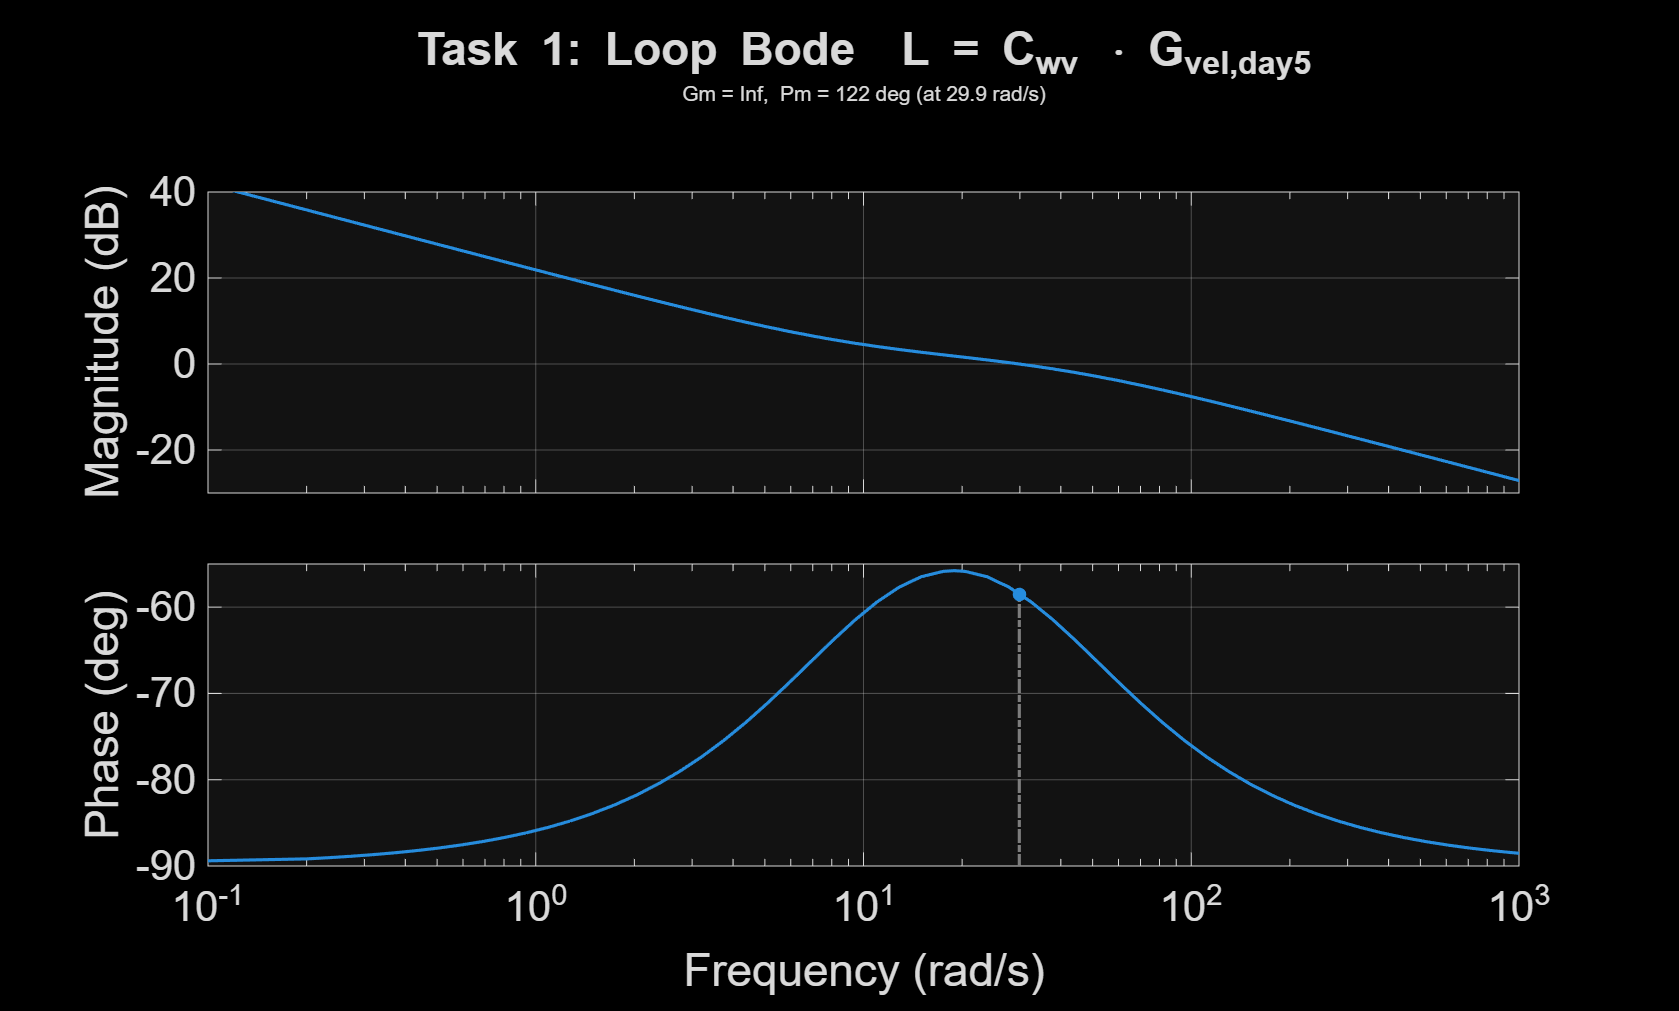
\includegraphics[width=0.75\linewidth]{images/regbot_task1_bode.png}
    \caption{Task 1 open-loop Bode plot $L_{wv}(s) = C_{wv}(s) G_{vel}(s)$ with phase and gain margins annotated.}
    \label{fig:task1_bode}
\end{figure}

\begin{figure}[H]
    \centering
    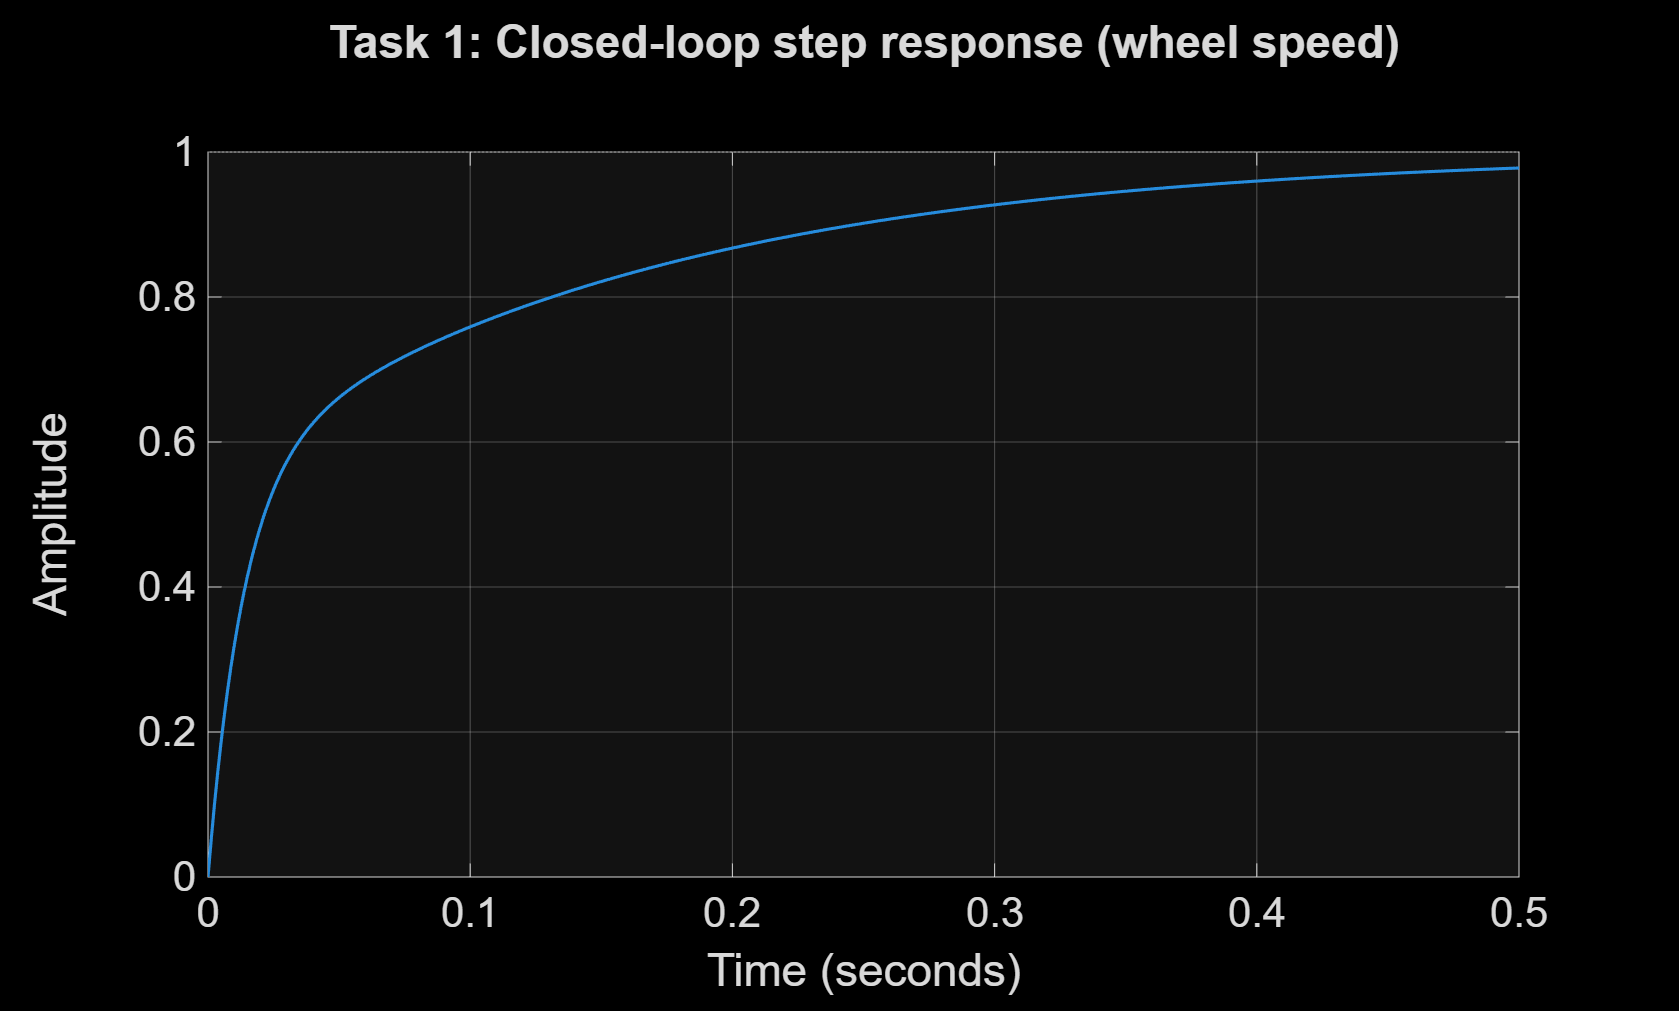
\includegraphics[width=0.75\linewidth]{images/regbot_task1_step.png}
    \caption{Task 1 closed-loop step response from the designed PI controller. The response converges to the reference without overshoot, confirming zero steady-state error.}
    \label{fig:task1_step}
\end{figure}

\subsection{Simulink Implementation}
The designed gains are assigned to the Simulink starter model variables \texttt{Kpwv = 3.31} and \texttt{tiwv = 0.10}\,s, replacing the default sample values provided with the model. This ensures the inner velocity loop in the Simscape Multibody model uses the Task 1 design for all subsequent experiments.

\subsection{Comments}
The achieved phase margin of $121.6^\circ$ is far above the $60^\circ$ specification, making the controller very robust but slightly conservative. A higher crossover frequency would give a faster response at the expense of phase margin. The current design is intentionally conservative to make the inner loop predictable for the outer balance controller, and the step response in Figure~\ref{fig:task1_step} shows a rise time of roughly $80\,\mathrm{ms}$ with no overshoot.

REGBOT experiment data will be added after the physical test.
